% Section content template for individual Educative lessons
% This file contains the actual content for a specific section
% Generated from Educative API section content

% Section: Sequence Diagram for LinkedIn
% Section ID: 4668575836274688
% Section Slug: sequence-diagram-for-linkedin
% Generated: 2025-12-14T13:35:17.411422

Sequence diagrams are an effective way to visualize the interactions between different entities and objects within a system. We can create different sequence diagrams for LinkedIn. In this lesson, we'll create sequence diagrams for the following interaction:

\begin{itemize}
\item
\protect\phantomsection\label{aPPYiggvK6JDX1jZ76IMn}
\textbf{Send a connection invitation:} A user sends a connection invitation to another user.
\end{itemize}

\subsection{Send a connection invitation}\label{N5DAhn1RKu-M4SDjz6H0I}
\\
The sequence diagram for sending a connection invitation should have the following actors and objects that will interact with each other:

\begin{itemize}
\item
\protect\phantomsection\label{FoKqCJoeMQZz8bhsTu7SU}
\textbf{Actors:}~\texttt{UserA}~and~\texttt{UserB}
\item
\protect\phantomsection\label{gXIc8E9bHuWWP_UcfzjtL}
\textbf{Objects:}~\texttt{Search}, \texttt{Notification}, and~\texttt{ConnectionInvitation}
\end{itemize}
\\
Here are the steps for sending a connection invitation interaction:

\begin{enumerate}
\item
User A searches for User B using the search service.
\item
If User B is found:

\begin{enumerate}
\item
The search service returns User B.
\item
A notification is sent to User B, indicating that they have appeared in a search.
\item
User A creates a new connection invitation object for User B.
\item
The connection invitation is sent from User A to User B.
\item
A notification is sent to User B informing them of the connection request.
\end{enumerate}
\end{enumerate}
\\
Based on the order above, the sequence diagram for sending a connection invitation on LinkedIn is given below:

\begin{figure}[htbp]
 \centering
 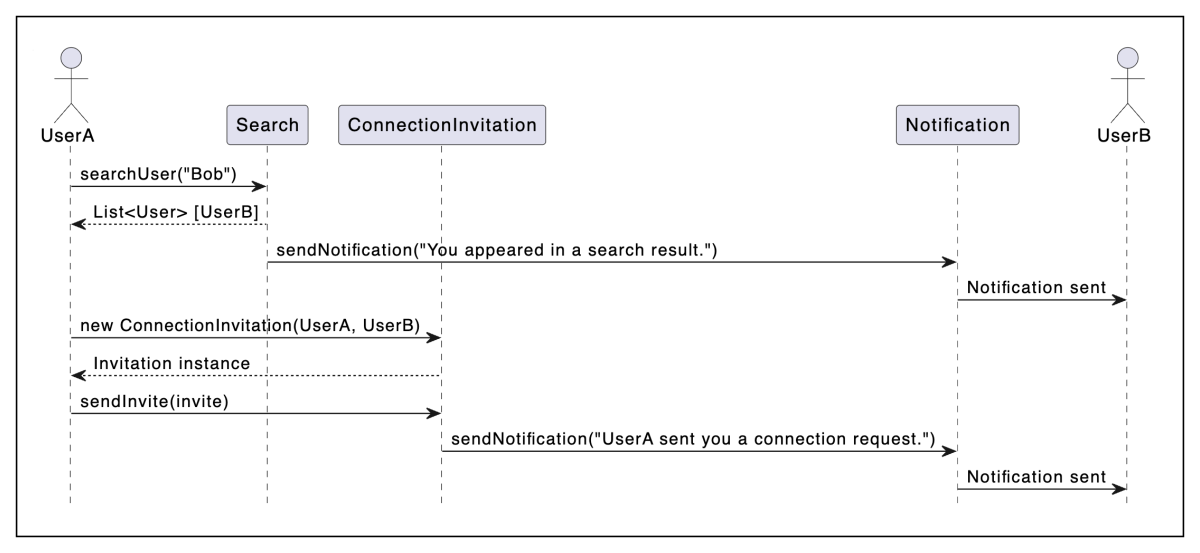
\includegraphics[width=0.5\textwidth]{Images/chapter_27/section_4668575836274688/6448555861344256.png}
 \caption{The sequence diagram for sending a connection invitation}
\end{figure}

Next, let's examine the activity diagrams for LinkedIn to understand the system's control flow.

% End of section content